

\begin{figure}
	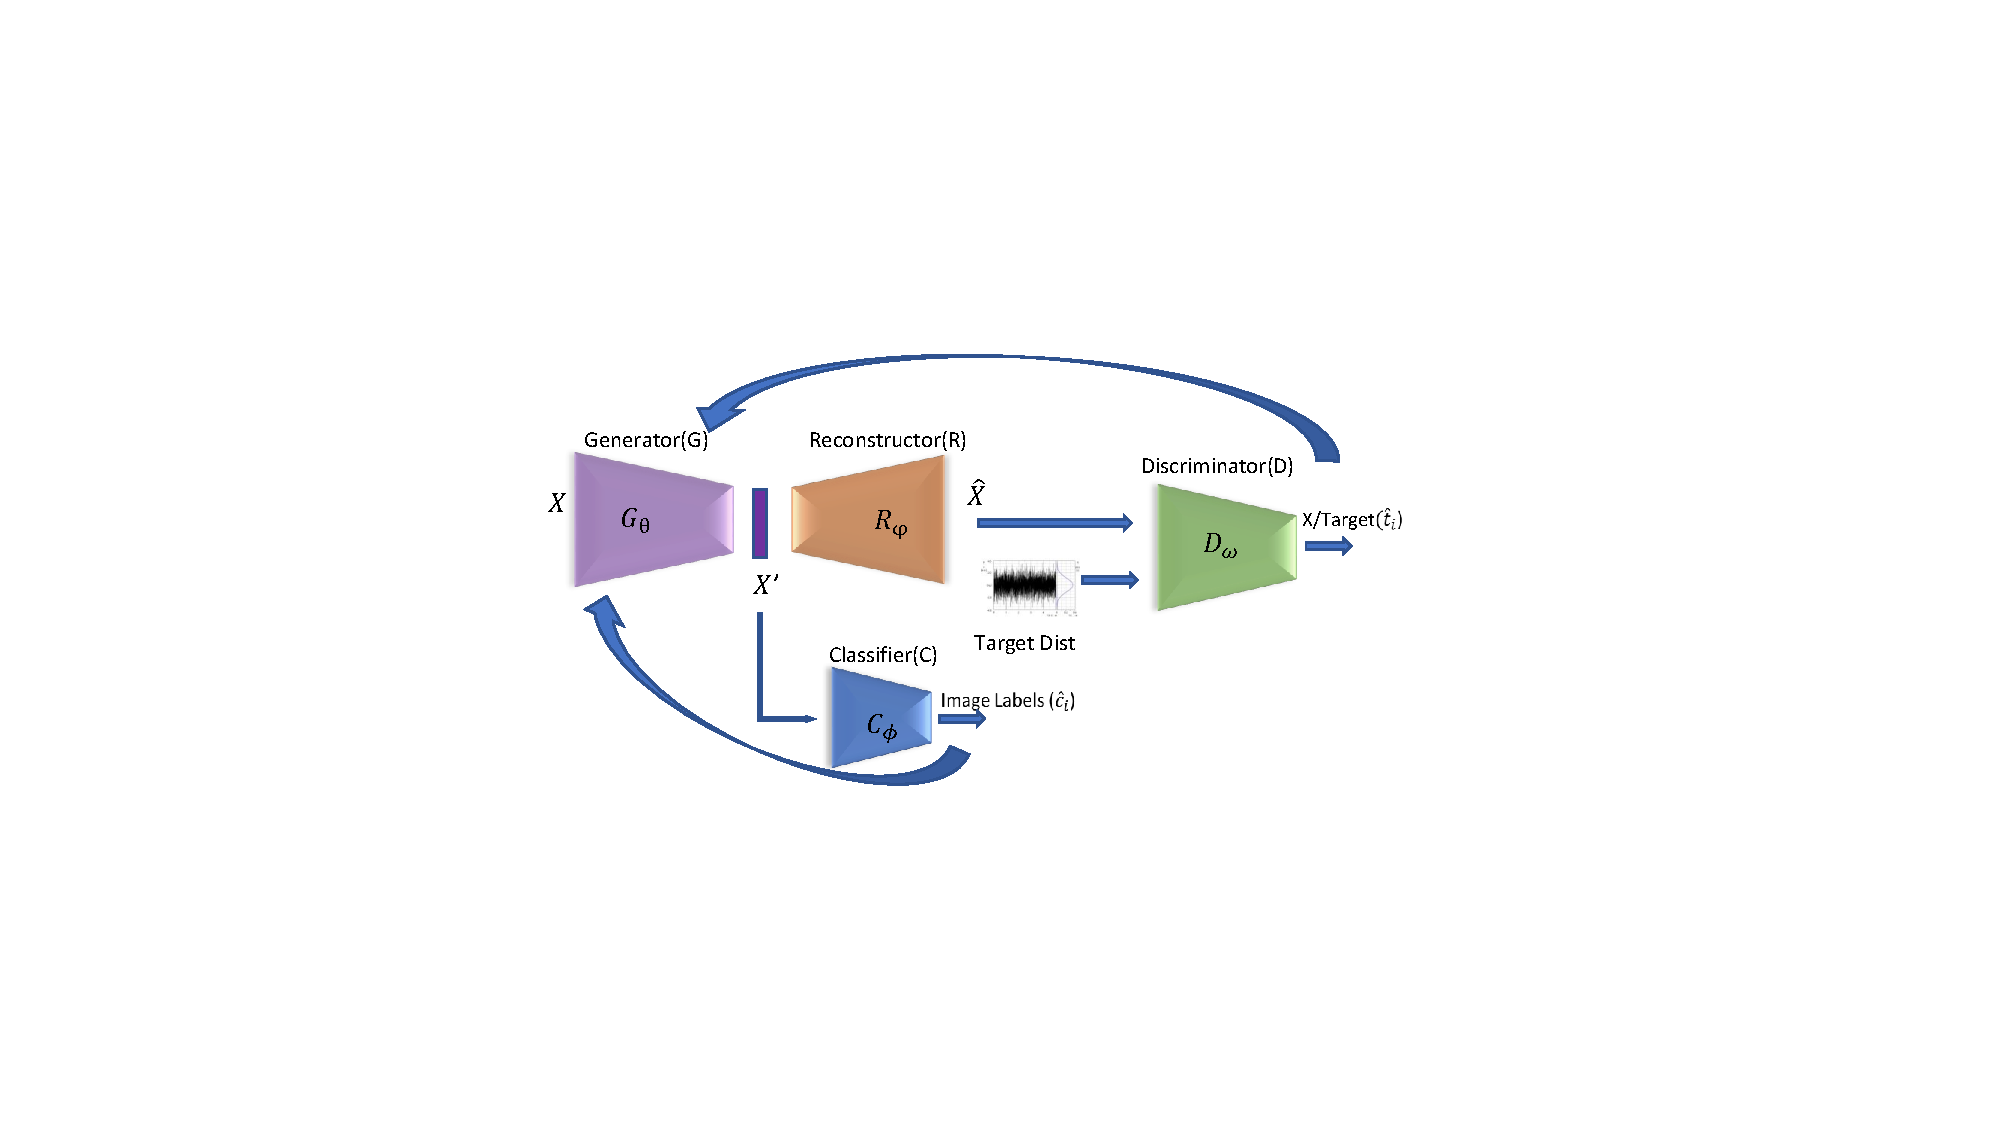
\includegraphics[width=\linewidth, trim= 8.5cm 5.5cm 8.5cm 5.5cm, clip=true]{\ChapterPathAutoGAN/figures/eGAN}
	\caption{AutoGAN-DRP}
	\label{fig:eGAN}
\end{figure}


\subsection{AutoGAN Dimension Reduction for Privacy Preserving}

We propose a deep learning framework for transforming face images to low dimensional data which is hard to be fully reconstructed. The framework can be presented in Figure \ref{fig:eGAN}. We leverage the structure of an auto-encoder \cite{Baldi2012} which contains encoder and decoder (in this work, we called them generator and re-constructor) in order to reduce data dimension. More specifically, the low dimensional representations are extracted from the middle layer of the auto-encoder (the output of the generator). The dimension-reduced data can be sent to the authentication server as an authentication request. We consider an adversary as a re-constructor implemented by a decoder. To resist against fully reconstructing images, the framework utilizes a discriminator in GAN \cite{Goodfellow2014} to direct reconstructed data to a designated target distribution with an assumption that the target distribution is different from our data distribution. In this work, the target distribution is sampled from Gaussian distribution and the mean is the average of training data. After projecting data into a lower dimension domain, the re-constructor is only able to partially reconstruct the data. Therefore, the adversary might not be able to recognize an individual's identity. To maintain data utility, we also use feedback from a classifier. The entire framework is designed to enlarge the distance between original data and its reconstruction to preserve individual privacy and retain significant data information. The dimension-reduced transformation model is extracted from the framework and provided to clients for reducing their face image dimensions. The classification model will be used in an authentication center that classifies whether a member's request is valid to have access (1) or not (0). 
 
We formulate the problem as follows:
Let $X$ be the public training dataset. $(x_i, y_i)$ is the $i$th sample in the dataset in which each sample $x_i$ has $d$ features and a ground truth label $y_i$. The system is aimed at learning a dimension reduction transformation $F(\cdot)$ which transforms the data from $d$ dimensions to $d'$ dimensions in which $d' \ll d $. Let $X'$ be the dataset in lower dimension domain. The dimension-reduced data should keep significant information to work with different types of machine learning tasks and should resist against the reconstruction or inference from data owner information.   

Our proposed framework is designed to learn a DR function $F(\cdot)$ that projects data onto low dimension space and preserves privacy at certain value of $\epsilon$. The larger distance implies higher level of privacy. Figure \ref{fig:eGAN} presents our learning system in which the dimension-reduced data $X'$ is given by a generator $G$. Since $X'$ is expected to be accurately classified by a classifier $C$, the generator improves by receiving feedback from the classifier via the classifier's loss function $\mathcal{L}_C$. We use a binary classifier for single-level authentication system and multi-class classifiers for multi-level authentication system. The classifier loss function is defined as the cross entropy loss of the ground truth label $y$ and predicted label $\hat y$ as follows.

\begin{equation}
\mathcal{L}_C=-\sum_{i=1}^n\sum_{j=1}^m y_{ij} \log(\hat y_{ij})  
%\quad y,\hat y \in \{0,1,..,m-1\}
\label{C_loss}
\end{equation}
where $m$ denotes the number of classes and $n$ denotes the number of samples.

To evaluate data reconstruction and enlarge the reconstruction distance, a re-constructor $R$ is trained as a decoder in an auto-encoder and sends feedback to the generator via its loss function $\mathcal{L}_R$. The re-constructor plays its role as an aggressive adversary attempting to reconstruct original data by using known data. The loss function of $R$ is the mean square error of original training data ($x$) and reconstructed data ($\hat x$), as displayed in (\ref{R_loss}) as follows 

\begin{align}
\mathcal{L}_R = \sum_{i=1}^n{(x_i - \hat x_i)^2} 
\label{R_loss}
\end{align}   
 
To direct the reconstructed data to a direction that reveals less visual information, the generator is trained with a discriminator $D$ as a minimax game in GAN. The motivation is to direct reconstructed data to a certain target distribution (e.g., normal distribution). To ensure a distance, the target distribution should be different to training data distribution. The discriminator aims to differentiate the reconstructed data from samples of the target distribution. The loss function of $D$ ($\mathcal{L}_D$) can be defined as a cross-entropy loss of ground truth labels (0 or 1) $t$ and prediction labels $\hat t$ shown in (\ref{D_loss}).

\begin{equation}
\mathcal{L}_D = -\sum_{i=1}^n{(t_i\log(\hat t_i) + (1 - t_i)\log(1 - \hat t_i))} 
\label{D_loss}
\end{equation}

The optimal generator parameter $\theta^*$ is given by the optimization problem of the generator loss function  $\mathcal{L}_G$:
\begin{equation}
\underset{\theta}{minimize} \; \mathcal{L}_G(\theta) = \alpha \min\limits_{\phi}{\mathcal{L}_C} - \beta\min\limits_{\omega}{\mathcal{L}_D}
 -\gamma\min\limits_{\varphi}{\mathcal{L}_R} + \mathcal{C}(\epsilon)
 \label{eqn:G_loss}
\end{equation}  
where $\theta$, $\phi$, $\omega$, and $\varphi$ are the model parameters of the generator, classifier, discriminator, and re-constructor respectively. $\alpha$, $\beta$, and $\gamma$ are weights of components in the objective function of the generator and can be freely tuned. $\mathcal{C}(\epsilon)$ is a constraint function with respect to hyper-parameter $\epsilon$, as to be elaborated in the following subsection.

\subsection{Optimization with Constraint}
In order to meet a certain level of reconstruction distance, we consider the constrained problem:

\begin{equation}
\begin{array}{l}
\; \; \; \;\underset{\theta}{minimize} \;\mathcal{L}_G(\theta) \\ 
s.t \; \; \;  \mathbb{E}_{x \sim p_d}[dist(x, \hat{x})] \leq \epsilon  
\end{array}
\label{constr}
\end{equation}

The optimization problem above can be approximated as an unconstrained problem \cite{pauljensen}:
\begin{equation} 
\underset{\theta}{minimize} \; ( \mathcal{L}_G(\theta) + \gamma \mathcal{C}(\epsilon) )  
\end{equation}
 where $\gamma$ is a penalty parameter and $\mathcal{C}$ is a penalty function 

\begin{equation} 
\mathcal{C}(\epsilon) = \max(0, \mathbb{E}_{x \sim p_d}[dist(x, \hat{x})] -\epsilon)
\end{equation}
Note that $\mathcal{C}$ is nonnegative, and $\mathcal{C}(\theta)=0$ iff the constraint in (\ref{constr}) is satisfied.


\subsection{Training Algorithms}


\begin{algorithm}[h]
	\caption{Algorithm for stochastic gradient descent training of $\epsilon$ -DR Privacy.}
	\begin{algorithmic}[1]
		\renewcommand{\algorithmicrequire}{\textbf{Input:}}
		\renewcommand{\algorithmicensure}{\textbf{Output:}}
		\REQUIRE Training dataset $X$. \\Parameter: learning rate $\alpha_r,\alpha_d,\alpha_c,\alpha_g $, 
		training steps $n_r,n_d,n_c,n_g$ \\
		A constraint for $\epsilon$-DR 
		\ENSURE  Transformation Model
		\\ \textit{Initialization.} 
		\FOR {$n$ global training iterations}
		\STATE  Randomly sample a mini batch from target distribution and label $\boldsymbol{t}$.\\
		\STATE  Randomly sample mini batch of data $\boldsymbol x $ and corresponding label $\boldsymbol{y}$  
		
		\FOR{$i = 0 $ to $n_r$ iterations}
		\STATE	Update the Reconstruction:\\
		$ \varphi_{i+1} = \varphi_{i} - \alpha_r \nabla_\varphi{\mathcal{L}_R(\varphi_{i} ,\boldsymbol{x} ) }	$\\
		\ENDFOR	
		\FOR{$j = 0 $ to $n_d$ iterations}
		\STATE	Update the Discriminator parameter:\\
		$ \omega_{j+1} = \omega_{j} - \alpha_d \nabla_\omega{\mathcal{L}_D(\omega_{j} ,\boldsymbol{x,t} ) }	$
		\ENDFOR	
		\FOR{$k = 0 $ to $n_c$ iterations}
		\STATE	Update the Classifier parameter:\\
		$ \phi_{k+1} = \phi_{k} - \alpha_c \nabla_\phi{\mathcal{L}_C(\phi_{k} ,\boldsymbol{x,y} ) }	$
		\ENDFOR	
		\FOR{$l = 0 $ to $n_g$ iterations}
		\STATE	Update the Generator parameter:\\
		$\theta_{l+1} = \theta_{l} - \alpha_g \nabla_\theta{\mathcal{L}_G(\theta_{l} ,\boldsymbol{x,t,y} ) }$
		\ENDFOR					
		\ENDFOR
		
		\RETURN 
	\end{algorithmic}
	\label{alg}
\end{algorithm}


Algorithm \ref{alg} describes the training process of AutoGAN-DRP. The framework contains four components, and they are trained one by one (lines 4-15) within one global training step. After sampling batches from target distribution and data for inputs of the models (lines 2-3), we  then train the four components. First, the re-constructor is trained in $n_r$ iterations while other components' parameters are fixed (lines 4-6). Second, the discriminator is trained (lines 7-9). Third, the classifier is trained in $n_c$ iterations (lines 10-12). Fourth, the generator is trained in $n_g$ iterations (lines 13-15). After training each component in their number of local training steps, the above training process is repeated until it reaches the number of global training iterations (lines 1-16). In our setting, the numbers of local training iterations ($n_c$, $n_r$, $n_d$, $n_g$ ) are much smaller than the number of global iterations $n$.   





